% Created 2020-12-07 Mon 14:27
% Intended LaTeX compiler: pdflatex
\documentclass[11pt]{article}
\usepackage[utf8]{inputenc}
\usepackage[T1]{fontenc}
\usepackage{graphicx}
\usepackage{grffile}
\usepackage{longtable}
\usepackage{wrapfig}
\usepackage{rotating}
\usepackage[normalem]{ulem}
\usepackage{amsmath}
\usepackage{textcomp}
\usepackage{amssymb}
\usepackage{capt-of}
\usepackage{hyperref}
\usepackage{cleveref}
\hypersetup{hidelinks=true}
\author{Stefano Ghirlanda}
\date{\today}
\title{The Tolman Mechanism\\\medskip
\large Development Notes}
\begin{document}

\maketitle

\section{Rationale}
\label{sec:orgd4d25c2}

\begin{itemize}
\item The Tolman mechanism implements a learning mechanism that formalizes
common theorizing in animal cognition.
\item The animal is assumed to build a mental model of its environment.
\item The model is then used to plan how to reach states with high value.
\item There are major computational challenges in such a mechanism and it
is unlikely that animals (or even people) can apply this strategy
in cases beyond a certain complexity.
\item We restrict the mechanism to work in worlds with a single goal, and
that ``restart'' after the goal is obtained.
\end{itemize}

\section{Variables}
\label{sec:org1b3a1dd}

\begin{itemize}
\item The Tolman mechanism learns \(S\to B\to S'\) transition
probabilities.
\item These estimates are called \(z(S,B,S')\).
\item Everything else is decided when responding.
\end{itemize}

\section{Learning}
\label{sec:org45913e8}

\begin{itemize}
\item There is a single learning rate, \(\alpha_z\).

\item Imagine first that all stimuli are made of a single element. When
\(S\to\ B\to S'\) is observed, \(z(S,B,X)\) is updated for all
\(X\) as follows:
\begin{equation}
  \label{eq:sbs-update}
  \Delta z(S,B,X) = \alpha_z \left( \lambda_{X} - z(S,B,X) \right)
\end{equation}
where \(\lambda_{X}=1\) when \(X=S'\) (the state that actually
occurred), and 0 for all other states.

\item With sufficient experience and sufficiently small \(\alpha_z\),
\cref{eq:sbs-update} will converge to the actual transition
probabilities.

\item How to extend to stimuli with more elements? Let's first consider
that all intensities are \(=1\). We can use
\begin{equation}
  \label{eq:sbs-multi}
  \forall S_j': \quad z(S,B,S_j') = \sum_{i=1}^n z(S_i,B,S_j')
\end{equation}
where the \(S_i\) are the elements of \(S\) and the \(S_j'\) the elements
of \(S'\). According to \cref{eq:sbs-multi}, different elements of \(S\)
compete for predicting each element of \(S'\) in the same way as they
would compete for accruing \(v\) or \(w\) values in A-learning (and
other mechanisms).

\item Using \cref{eq:sbs-multi} to calculate \(z(S_i\ldots S_n,B,S_i')\) we can
update each \(S_i\) as follows:
\begin{equation}
  \label{eq:sbs-update}
  \Delta z(S_i,B,X) = \alpha_z \left( \lambda_X - z(S,B,S_j') \right)
\end{equation}
where \(\lambda=1\) if \(X\in S'\) and \(\lambda=0\) otherwise.

\item With intensities written as \(x\) we can use:
\begin{equation}
  \label{eq:sbs-multi-intensity}
  \forall S_j': \quad z(S,B,S_j') = \sum_{i=1}^n z(S_i,B,S_j')x_i
\end{equation}
\begin{equation}
  \label{eq:sbs-update-intensity}
  \Delta z(S_i,B,S_j') = \alpha_z \left( \lambda_X - z(S,B,S_j') \right) x_i x'_j
\end{equation}
\end{itemize}

\subsection{Trial implementation \textit{<2020-12-07 Mon>}}
\label{sec:org81cc5f6}

\begin{itemize}
\item The equations above have been implemented in the \texttt{github} branch
\texttt{tolman-mechanism}

\item I have made a super simple test where there is only behavior \(B\) and
two stimuli \(S_1\) and \(S_2\)), and the only thing that happens is the
sequence:
\begin{equation}
  \label{eq:simple-test}
  \cdots \to S_1 \to B \to S_2 \to B \to S_1 \to \cdots
\end{equation}

\item In this case, the Tolman mechanism should learn:
\begin{align}
  \label{eq:simple-test-z}
  z(S_1,B,S_2) &= 1\\
  z(S_1,B,S_1) &= 0\\
  z(S_2,B,S_1) &= 1\\
  z(S_2,B,S_2) &= 0
\end{align}

\item Printing this values throughout the simulation shows that they are
in fact learned, but the graphs do not come out well. I think this
is because the current plotting code only updates the plot for
stimulus elements that are actually presented, but the Tolman
mechanism also updates \(z(S,B,S')\) for \(S'\) elements that are not
present. For example, this is a graph I get:
\end{itemize}
\begin{center}
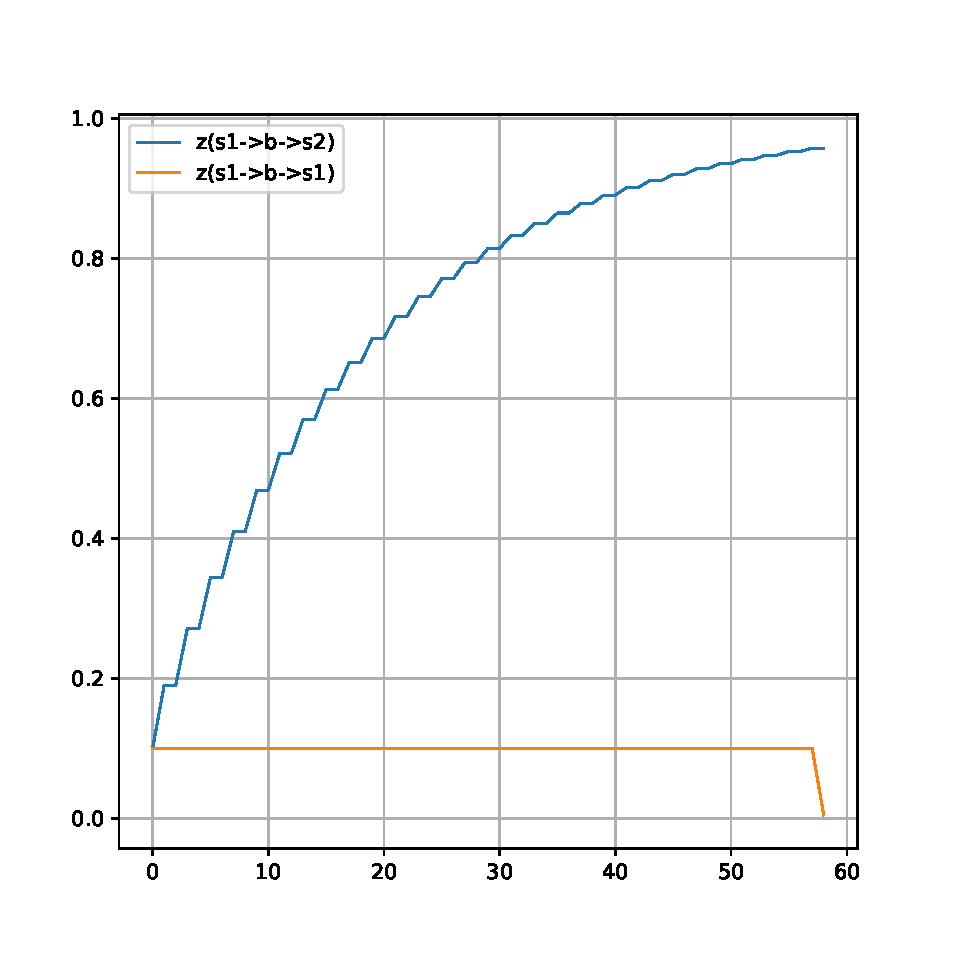
\includegraphics[width=.5\textwidth]{./first-try.pdf}
\end{center}

\begin{itemize}
\item The initial values of all \(z\) is 0.1 for testing purposes. The blue
line goes to 1 as it should. The orange is plotted at the initial
0.1 throughout the simulation, but for the last point, which is the
correct value of 0. As I mentioned above, however, if I print the
values during learning I do see that they are decreasing toward 0
all the time.

\item (Element intensities and multiple elements are implemented but not
tested yet.)
\end{itemize}

\section{Responding}
\label{sec:orgf30a6be}

\begin{itemize}
\item Responding assumes that the world model in \(z\) is true.

\item Responding should then make the ``best plan'' given this
knowledge.

\item Evaluating all possible plans is tricky in general. Let's work with
a particular kind of world to begin with:
\begin{enumerate}
\item There is only one valued stimulus, called the goal.
\item When the goal is reached, the next state is determined by the
world using a fixed rule (deterministic or stochastic).
\end{enumerate}

\item The second condition means that we need to consider just how to
reach the goal once, since after that the world ``resets'' to a
statistically equivalent state.

\item The first step is to find all paths to the goal. We start from the
goal and we go backwards along possible transitions, that is, all
transitions with \(z>0\) for some \(B\). If we eventually reach the
current state, we store the sequence of transitions and call it a
``path.''

\item We calculate the expected \emph{rate} of return for all paths to the
goal, that is the expected value divided the path length (number of
actions):
\end{itemize}
\begin{equation}
  \label{eq:path-value}
  v(\mathrm{path}) = \frac{ u(S_\mathrm{goal}) -\sum_{B\in\mathrm{path}} c(B)}{ l_\mathrm{path} } \prod_{S'\in\mathrm{path}} \Pr(S\to B\to S') 
\end{equation}

\begin{itemize}
\item In \cref{eq:path-value}, the sum is over all behaviors in the path,
\(l_\mathrm{path}\) is path length, and the product is over all
transition probabilities in the path. (This is the probability that
the plan will succeed.)

\item We then give a value to each behavior that is feasible in response
to the current stimulus. If the behavior is the first step on a path
to the goal, its value is the \(v\) value of the goal. If it is not,
its value is \texttt{start\_v}.

\item If a behavior is the first on more than one path, we can average the
\(v\)'s using the success probability of each path, so we should store
these somewhere.

\item We then use softmax to choose a behavior.
\end{itemize}
\end{document}